\documentclass[document.tex]{subfiles} 
\begin{document}

\chapter{معمارية حواسيب \en{x86}}
حواسيب عائلة \cmd{x86} تتبع لمعمارية العالم جون نويمان (\en{John von Neumann architecture}) والتي تنص على أن أي تصميم لجهاز حاسب يجب أن يتكون من الثلاث وحدات التالية :
\begin{enumerate}
\item معالج أو وحدة معالجة مركزية (\en{Central Processing Unit}).
\item ذاكرة (\en{Memory}).
\item أجهزة إدخال وإخراج (\en{I/O Devices}).
\end{enumerate}

\textbf{الوحدة الاولى} هي وحدة المعالجة والتي تقوم بتنفيذ الأوامر والعمليات الحسابية ، أما \textbf{الوحدة الثانية} فهي تحوي البيانات والتعليمات والأوامر التي يجب لوحدة المعالجة أن تنفذها ، \textbf{وأخيراً} وحدات الإدخال والإخراج وهي الاجهزة التي تستخدم في ادخال البيانات واخراجها.(انظر الشكل \ref{fig:vonarch} حيث يوضح مثالاً لهذه المعمارية) ويربط بين كل هذه الأجزاء هو مسار النظام (\en{System Bus}) وفيما يلي سنستعرض وظيفة كل جزء على حدة.

\begin{figure}[h!]
  \caption{معمارية حواسيب \en{x86}}
  \centering
   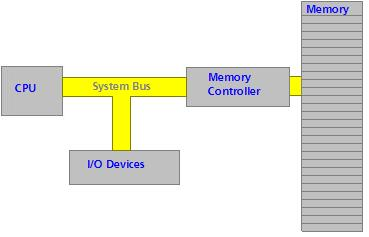
\includegraphics[width=0.7\textwidth]{../img/vonarch}
 \label{fig:vonarch} 
\end{figure}

\section{معمارية النظام}
\subsection{مسار النظام \en{System Bus}}
يربط مسار النظام (\en{System Bus}) \footnote{ويسمى أيضا \en{Front-side Bus}.} وحدة المعالجة المركزية (\en{CPU}) مع متحكم الذاكرة الرئيسية . وظيفة هذه المسارات هي نقل البيانات بين أجزاء الحاسب المختلفة. والشكل \ref{fig:fsb} يوضح الصورة العامة للمسارات في أجهزة الحواسيب الشخصية (\en{Personal Computers}). ويتألف مسار النظام من ثلاث مسارات وهي مسار البيانات (\en{Data Bus}) ومسار العناوين (\en{Address Bus}) ومسار التحكم (\en{Control Bus}).


\begin{figure}[h!]
  \caption{المسارات في الحواسيب الشخصية \en{x86}}
  \centering
   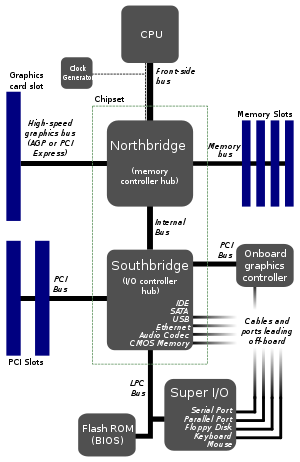
\includegraphics[width=0.5\textwidth]{../img/fsb}
  \label{fig:fsb} 
\end{figure}

\subsubsection{مسار البيانات \en{Data Bus}}
مسار البيانات هو عبارة عن خطوط (\en{Lines}) كل خط يمثل بت واحد. وغالبا ما يكون هناك \cmd{32} خط (أي أن مسار البيانات بطول \cmd{32-bit}) ويستخدم هذا المسار في نقل البيانات (\en{Data}) من المعالج (وتحديداً من وحدة التحكم \en{Control Unit}) الى متحكم الذاكرة (الى الجسر الشمالي \en{NorthBridge} تحديدا نظراّ لان متحكم الذاكرة يطبق على عليه). وبسبب أن حجم مسار البيانات هو حجم ثابت فان هذا يتطلب معالجة خاصة عند ارسال بيانات بطول أقل من طول مسار البيانات ، فغالبا ما يقوم المعالج باضافة أصفار في الخطوط الغير مستخدمة (\en{Padding}). أما في حالة إرسال بيانات بطول أكبر فان عملية نقلها تتم على عدة مراحل وفي كل مرحلة ترسل \cmd{32-bit} من البيانات .

\subsubsection{مسار العناوين \en{Address Bus}}
يستخدم مسار العناوين في نقل عنوان الذاكرة المراد استخدامه سواءاً للقراءة منه أو الكتابة عليه ، ويحدد حجم مسار العناوين أكبر عنوان يمكن الوصل اليه في الذاكرة وبالتالي يحدد لنا حجم الذاكرة التي يستطيع الحاسب التعامل معها . وفي الأجهزة التي تستخدم معالجات انتل \en{8086} كان حجم هذا المسار هو \cmd{20-bit} وبالتالي فان أقصى ذاكرة يتعامل معها هذا المعالج هي \cmd{1 MB}\footnote{ناتجة من حساب \cmd{2} مرفوع للقوة \cmd{20}.} أما في معالجات \en{80286/80386} فان حجم هذا مسار هو \cmd{24-bit} وفي المعالجات التي تليها تم زيادة هذا الحجم الى \cmd{32-bit} وبالتالي يمكن تنصيب ذاكرة بحجم \cmd{4 GB} ، وفي المعالجات الحديثة تم زيادة هذا الحجم ، ولكننا سنقتصر في هذا البحث على المعالجات التي تدعم مسار عناوين بطول \cmd{32-bit} بسبب انتشارها وسيطرتها لمدة من الزمن على أجهزة الحواسيب الشخصية.

\subsubsection{مسار التحكم \en{Control Bus}}
يستخدم مسار التحكم في ارسال الأوامر مثل أمر القراءة من العنوان الموجود على مسار العناوين أو أمر الكتابة على العنوان المطلوب . ويتألف هذا المسار من عدد من الخطوط وكل خط (بت) يؤدي وظيفة محددة. أحد هذه الخطوط هو خط الكتابة \cmd{WRITE} والذي يعني أن العنوان الموجود على خط العناوين يجب أن تُعيَّن له القيمة الموجودة في مسار البيانات . الخط الآخر هو خط القراءة \cmd{READ} والذي يدل على أن العنوان الموجود في مسار العناوين يجب أن تُقرأ قيمته الى مسار البيانات . آخر خط يهمنا هو خط الولوج \cmd{ACCESS} والذي يحدد ما اذا كان العنوان موجهٌ الى متحكم الذاكرة أم الى متحكم  الإدخال والإخراج وفي حالة كانت قيمة هذا الخط هي القيمة \cmd{1} فان هذا يعني أن العنوان موجهُ الى متحكم أجهزة الإدخال والإخراج وبالتالي سيتم القراءة من هذا العنوان أو الكتابة اليه وذلك بحسب قيمة الخطين \cmd{READ and WRITE}.

\subsection{متحكم الذاكرة}
قبل أن نذكر وظيفة هذا المتحكم يجب إعطاء نبذة عن ماهية المتحكمات (\en{Controllers}) في جهاز الحاسب. ويُعرَّف \textbf{المتحكم} بأنه شريحة تتحكم بعتاد ما تحوي العديد من المسجلات الداخلية وظيفتها هو استقبال الأوامر وتنفيذها على العتاد. ويمكن أن نعرفها بأنها شريحة للربط ما بين الأوامر البرمجية الى أوامر تنفذ على عتاد ما. وأي متحكم يحوي العديد من المسجلات سواءاً كانت لإرسال واستقبال البيانات أو للأوامر ، وأي مسجل يجب أن يأخذ رقم فريد يميزه عن بقية المسجلات الموجودة في هذا المتحكم أو في أي متحكم آخر وذلك حتى نتمكن من التعامل معه برمجياً ، هذا الرقم يعرف باسم المنفذ (\en{Port}) وسنطلع عليه لاحقاً. وعمل المتحكم يبدأ عندما يُرسل أمر اليه حيث يبدأ المتحكم في تنفيذ هذا الأمر ومن ثم يضع النتيجة في أحد مسجلاته ويرسل إشارة (\en{Interrupt}) الى المعالج لكي يقوم بقرائة القيمة.

نعود الى متحكم الذاكرة الرئيسية والذي يتواجد غالبا على متحكم الجسر الشمالي (\en{NorthBridge}) إنظر الشكل \ref{fig:nbridge} .حيث تكمن وظيفته الأساسية في استقبال الأوامر المرسلة الى الذاكرة وتنفيذها ، ويقوم هذا المتحكم يتوجيه العناوين المرسلة الى أي من شرائح الذاكرة كذلك يقوم بإعادة تنعيش (\en{Refresh}) هذه الذاكرة طيلة عمل الحاسب حتى لا تفقد الذاكرة محتوياتها.

\begin{figure}[h!]
  \caption{الجسر الشمالي}
 {يعتبر هذا الجسر حلقة الوصل ما بين المعالج والذاكرة الرئيسية والبايوس وذاكرة الفيديو ومتحكم الإدخال والإخراج حيث يستقبل الأوامر ويقوم بتوجيهها الى المتحكم المطلوب.}
\\
  \centering
   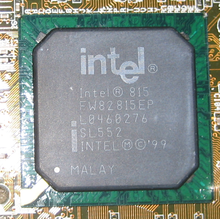
\includegraphics[width=0.2\textwidth]{../img/nbridge}
  \label{fig:nbridge} 
\end{figure}


\subsection{متحكم الإدخال والإخراج}
يستخدم متحكم  الإدخال والإخراج (ويسمى أيضا الجسر الجنوبي \en{SouthBridge}) في ربط متحكمات أجهزة الإدخال والإخراج مع المعالج وهذا يتضح من الشكل \ref{fig:fsb}. حيث يظهر أن الجسر الشمالي يرتبط مباشرة مع المعالج بينما الجسر الجنوبي يرتبط مع الجسر الشمالي والذي بدوره يربط متحكمات عتاد الإدخال والإخراج في الحاسب.
وكل جهاز يرتبط بالحاسب (مثل لوحة المفاتيح أو الفأرة أو الطابعة ...الخ) لديه متحكم بداخل الجهاز ومتحكم آخر بداخل الحاسب ، حيث يرسل المتحكم الموجود بداخل الحاسب الأوامر الى المتحكم الموجود بداخل العتاد . ولبرمجة أي جهاز فانه يجب برمجة المتحكم الموجود في الحاسب وهذا يتم عن طريق معرفة المسجلات (\en{Registers}) الموجودة به ووظيفة كل مسجل فيه حتى نتمكن من إرسال الأوامر الصحيحة اليه. هذه المسجلات تأخذ أرقاما معينة تسمى منافذ برمجية (\en{Software Ports})  بحيث تميز هذه الأرقام المسجلات من بعضها البعض\footnote{هناك بعض المسجلات لبعض المتحكمات تأخذ نفس الرقم ، لكن طبيعة الأمر المُرسل (قراءة أو كتابة) هو الذي يحدد المسجل الذي يجب التعامل معه.}.

\subsubsection{المنافذ \en{Ports}}
يستخدم مفهوم المنافذ في علوم الحاسب للدلالة على عدة أشياء فمثلا في مجال برمجة الشبكات تكون برامج الخادم لها رقم منفذ معين حتى تسمح لبرامج العميل بالاتصال معها، كذلك توجد المنافذ الموجودة في اللوحة الأم لوصل عتاد الحاسب بها ، أيضا أي مسجل في متحكم على الجهاز لديه رقم منفذ وهذا ما نقصده في حديثنا عن المنافذ في هذا البحث.
و يمكن الوصول لمنافذ المتحكمات والتي تعرف ب \en{I/O ports} باستخدام تعليمة المعالج \cmd{in port\_address} والتعليمة \cmd{out port\_address} حيث تستخدم الأولى لقراءة قيمة من مسجل في متحكم ووضعها في أحد مسجلات المعالج أما التعليمة الثانية تستخدم لكتابة قيمة في مسجل للمعالج الى مسجل في المتحكم . وعند استخدام أحد هذين الأمرين فان ذلك يعني أن العنوان موجه الى متحكم الإدخال والإخراج وليس الى متحكم الذاكرة حيث يقوم المعالج بتعين قيمة الخط \cmd{ACCESS} الموجود في مسار التحكم (\en{Control Bus})  وبالتالي يستجيب متحكم الإدخال والإخراج ويقرأ هذا العنوان ويقوم بتوجيهه الى المتحكم المطلوب . وهناك بعض الأجهزة تستخدم عنواين الذاكرة للوصول للمتحكم الخاص بها وهو ما يعرف ب \en{Memory Mapped I/O} حيث عند كتابة أي بيانات على هذه العناوين فان ذلك يعني كتابة هذه البيانات على متحكمات للأجهزة وليس على الذاكرة الرئيسية. فمثلاً عند الكتابة على عنوان الذاكرة \cmd{0xa000:0x0} فان هذا يؤدي الى الكتابة على شاشة الحاسب نظراً لان هذا العنوان هو موجه (\en{Memory Mapped}) مع متحكم شاشة الحاسب والجدول \ref{tbl:mem_map} يوضح خريطة الذاكرة في حواسيب \cmd{x86}، ولا تحتاج الكتابة لمثل هذه العناوين استخدام الأوامر \cmd{in/out} بعكس الكتابة في عنواين المنافذ \cmd{port I/O} .


\begin{table}
\caption{مخطط الذاكرة لحواسيب \en{x86}}
\centering
\begin{tabular}{ | r | r | r |}
\hline  
عنوان البداية & عنوان النهاية & الوصف \\
\hline \hline
\en{0x00000} & \en{0x003ff} & جدول المقاطعات \en{IVT} \\
\en{0x00400} & \en{0x004ff} & منطقة بيانات البايوس \\
\en{0x00500} & \en{0x07bff} & غير مستخدمة \\
\en{0x07c00} & \en{0x07dff} & برنامج محمل النظام \\
\en{0x07e00} & \en{0x9ffff} & غير مستخدمة \\
\en{0xa0000} & \en{0xaffff} & ذاكرة الفيديو \en{Video RAM} \\
\en{0xb0000} &\en{ 0xb7777} & ذاكرة الفيديو أحادية اللون \en{Monochrome VRAM} \\
\en{0xb8000} & \en{0xbffff} & ذاكرة الفيديو الملونة \en{Color VRAM} \\
\en{0xc0000} & \en{0xc7fff} & ذاكرة \en{Video ROM BIOS} \\
\en{0xc8000} & \en{0xeffff} & منطقة \en{BIOS Shadow Area} \\
\en{0xf0000} & \en{0xfffff} & نظام البايوس \\
 \hline  
\end{tabular}
\label{tbl:mem_map}
\end{table}

عناوين منافذ الإدخال والإخراج (\en{Port I/O}) هي عناوين تستخدمها المسجلات الموجودة على المتحكمات ويقوم البايوس بمهمة ترقيم هذه المسجلات ، والجدول \ref{tbl:io_map} يعرض قائمة بعناوين المنافذ ووظيفة كل منهم.
\begin{table}
\caption{منافذ الإدخال والإخراج لحواسيب \en{x86}}
\centering
\begin{tabular}{ | l | l |}
\hline  
رقم المنفذ & الإستخدام \\
\hline \hline
\en{0000-000f	} & \en{Slave DMA controller}\\
\en{0010-001F} & \en{System}\\
\en{0020-0021} & \en{First Interrupt controller (8259 chip)}\\
\en{0030-0031} & \en{Second interrupt controller}\\
\en{0040-0043} & \en{Programable Interval Timer 1 (8254 chip)}\\
\en{0048-004B} & \en{Programable Interval Timer 2}\\
\en{0050-006F} & \en{System devices}\\
\en{0070-0071} & \en{NMI Enable / Real Time Clock}\\
\en{0080-008B} & \en{DMA Page registers}\\
\en{0090-009F} & \en{System devices}\\
\en{00A0-00A1} & \en{Slave interrupt controller}\\
\en{00C0-00DE} & \en{Master DMA controller}\\
\en{00F0-00FF} & \en{System devices}\\
\en{0100-0167} & \en{System devices}\\
\en{0168-016F} & \en{IDE Interface - Quaternary channel}\\
\en{0170-0177} & \en{IDE interface - Secondary channel}\\
\en{01E8-01EF} & \en{IDE Interface - Tertiary channel}\\
\en{01F0-01F7} & \en{IDE interface - Primary channel}\\
\en{0200-0207} & \en{Games Port (joystick port)}\\
\en{0220-022F} & \en{Usually used by sound cards, also used by NOVEL NETWARE KEY CARD}\\
\en{0270-0273} & \en{Plug and Play hardware}\\
\en{0278-027A} & \en{Parallel  Port *}\\
\en{0280-028F} & \en{Sometimes used for LCD Display I/O}\\
\en{02B0-02DF} & \en{Alternate VGA Video Display Adaptor assignment (secondary address)}\\
\en{02E0-02E7} & \en{GPIB 0, data aquisition card 0 (02E1 to 02E3 only)}\\
\en{02E8-02EF} & \en{Serial Port - COM 4}\\
\en{02F8-02FF} & \en{Serial Port - COM 2}\\
\en{0300-031F} & \en{Often used as a default for Network Interface cards (was prototype card)}\\
\en{0320-023F} & \en{ST506 and ESDI Hard Disk Drive Interface (mostly used in PX/XT and early PC/AT)}\\
\en{0330-0331} & \en{MPU-401 (midi) interface, on Sound Cards }\\
\en{0360-036F} & \en{Sometimes used for Network Interface cards}\\
\en{0376-0377} & \en{Another address used by the Secondary IDE Controller (see 0170-0177)}\\
\en{0378-037A} & \en{Parallel Port *} \\
\en{0388-038B} & \en{FM (sound) synthesis port on sound cards}\\
\en{03B0-03BB} & \en{MDA, EGA and VGA  Video Display Adaptor  (only 03B0 to 03BB used)}\\
\en{03BC-03BF} & \en{Parallel Port (originally only fitted to IBM mono display adaptors) *}\\
\en{03C0-03DF} & \en{EGA / VGA Video Display Adaptor, (Primary address)}\\
\en{03E0-03E7} & \en{PCIC PCMCIA Port Controller}\\
\en{03E8-03EF} & \en{Serial Port - COM 3}\\
\en{03F0-03F6} & \en{Floppy Disk Drive Interface}\\
\en{03F7-03f7	} & \en{Another address used by the Primary IDE Controller (see 01F0-01F7)}\\
\en{03F8-03FF} & \en{Serial Port - COM 1}\\
\en{0533-0537} & \en{Windows sound system (used by many sound cards)}\\
\hline  
\end{tabular}
\label{tbl:io_map}
\end{table}

\section {المعالج}
يعتبر المعالج هو المحرك الرئيسي لجهاز الحاسب حيث يستقبل الأوامر ويقوم بتفيذها .

\subsection{دورة تنفيذ التعليمات} 
لكي يُنفذ المعالج البرامج الموجودة على الذاكرة فان هذا يتطلب بعضا من الخطوات التي يجب أن يقوم بها ، وفي كل دقة للساعة (\en{Clock tick}) يقوم المعالج بالبدء بخطوة من هذه الخطوات ، وفيما يلي سردا لها.
% راجع هذه المعلومات

\begin{description}
\item [أولاً] مرحلة جلب البيانات (\en{Fetch}) وفيها يتم جلب البيانات من الذاكرة الرئيسية الى المسجلات بداخل المعالج.
\item [ثانياً] مرحلة تفسير البيانات (\en{Decode}).
\item [ثالثاً] مرحلة تنفيذ البيانات (\en{Execute}).
\item [رابعاً] مرحلة حفظ النتائج (\en{Write back}).
\end{description}

\subsection{أنماط عمل المعالج \en{CPU Modes}}
عندما طرحت شركة أنتل أول اصدارة من معالجات \cmd{16-bit} لم يكن هناك ما يعرف بأنماط المعالج حيث كان المعالج يعمل بنمط واحد وهو ما يعرف الان بالنمط الحقيقي (\en{Real Mode}) ، في هذا النمط يقوم المعالج بتنفيذ أي أمر موجه اليه ولا يوجد ما يُعرف بصلاحيات التنفيذ حيث يمكن لبرنامج للمستخدم أي يقوم بتنفيذ أمر يتسبب في ايقاف النظام عن العمل (مثل الأمر \cmd{hlt}) ، كذلك توجد عددٌ من المشاكل في هذا النمط فمثلا لا توجد حماية للذاكرة من برمجيات المستخدم ولا يوجد أي دعم لمفهوم تعدد المهام (\en{Multitasking}). لذلك سارعت أنتل بادخال عدة أنماط على بنية المعالج لتحل هذه المشاكل ، بحيث يُمكن للمعالج أي يعمل في أي نمط وأن يقوم بالتحويل وقتما شاء. ويُعرَّف \textbf{نمط المعالج} بأنه طريقة معينة يتبعها المعالج أثناء عمله لتنفيذ الأوامر فمثلا يحدد النمط المستخدم ما إذا كان هناك حماية لعنواين الذاكرة بحيث لا يمكن لبرنامج لا يمتلك صلاحيات معينة الوصول لأي منطقة في الذاكرة. 

\subsection{النمط الحقيقي \en{Real Mode}}
هذا النمط هو الذي يبدأ الجهاز الحاسب بالعمل عندما يقلع وهذا بسبب أن حواسيب \cmd{x86} تم تصميمها بحيث تدعم الأجهزة القديمة وحتى تحافظ انتل على ذلك فان هذا ما جعلها تدع المعالج يبدأ بالنمط الحقيقي عند الإقلاع توافقاً مع الحواسيب القديمة ، وبعد ذلك عندما يستلم نظام التشغيل زمام التحكم بالحاسب فانه مخيرٌ ما بين الإستمرار بالعمل في هذا النمط وبالتالي يسمى هذا النظام \textbf{نظام تشغيل \en{16-bit}} وبين تحويل نمط المعالج الى النمط الاخر وهو النمط المحمي (\en{Protected Mode}) وبالتالي يسمى النظام \textbf{نظام تشغيل \en{32-bit}}.
في هذا النمط يستخدم المعالج مسجلات من طول \cmd{16-bit} (مثلاً المسجلات \en{ax,bx,cx,dx,...etc}) ويستخدم عنونة \textbf{المقطع:الإزاحة} (\en{Segment:Offset}) للوصول الى الذاكرة الرئيسية - سيتم شرحها في الفقرة التالية- وأيضا يدعم ذاكرة بحجم \en{1} ميجابايت ولا يقدم أي دعم لحماية الذاكرة والذاكرة التخيلية (\en{Virtual Memory}) ولا يوفر حماية للذاكرة من برمجيات المستخدم.

\subsubsection{عنونة المقطع:الإزاحة (\en{Segment:Offset Addressing})}
بعد طرح أنتل لمعالج \en{8086} وهو أول معالج 16 بت ، ظهرت مشكلة حجم الذاكرة حيث أن طول المسجلات المستخدمة في هذا المعالج (مسجلات البيانات والعناوين) هو 16 بت وهذا ما سمح للمسجل بأن يتعامل مع  64 كيلوبايت فقط من الذاكرة على الرغم من أن مسار العناوين (\en{Address Bus}) في هذه الأجهزة  كان بحجم 20 بت وهو ما يسمح باستخدام ذاكرة بحجم 1 ميجا. الى هنا كان الخيار أمام شركة أنتل هو بزيادة حجم المسجلات الموجودة بداخل المعالج ولكن هذا الحل كان مكلفاً جدا آنذاك نظراً لإن هذه المسجلات هي ذواكر من النوع \en{SRAM} وهو نوع مكلفاّ على الرغم من إمكانياته العالية. ما فعلته انتل هو إيجاد طريقة مختلفة لعنونة الذاكرة فبدلاً من استخدام مسجل واحد للوصل الى عناوين الذاكرة تم استخدام مسجلين كل منهما بطول 16 بت ، الفكرة كانت في تقسيم الذاكرة الى مقاطع (\en{Segments}) ويُستخدم أحد المسجلات للدلالة على رقم أو عنوان المقطع (\en{Segment Number or Address}) وبالتالي هناك 65536 مقطع مختلف\footnote{هذا ناتج من حساب \en{$2^{16}$}.} ويُستخدم المسجل الآخر للوصل الى العناوين بداخل المقطع وهي ما تعرف بالقيم (\en{Offsets}) بداخل المقطع وبالتالي كل مقطع يحوي 65536 بايت (أي أن حجم المقطع هو 64 كيلوبايت).
إذاً يُعرَّف \textbf{المقطع \en{Segments}} بأنها منطقة من الذاكرة بحجم 64 كيلوبايت ويمكن الوصول الى أي مقطع وذلك بتحميل رقم المقطع أو عنوان المقطع الى أي من مسجلات المقاطع الموجودة بداخل المعالج (مثل المسجلات \cmd{CS,SS,DS,ES}) - سيتم شرحها لاحقا - ، ويمكن الوصول الى محتويات المقطع \textbf{الإزاحة \en{Offset}} وذلك بتحميل العنوان المطلوب الوصل اليه الى أي من مسجلات القيم (تبدأ العناوين في أي مقطع من العنوان \en{0x0} الى \en{0xffff}). هذه الطريقة التي اقترحتها انتل للوصول الى عناوين الذاكرة خلقت لنا مفهوم العنوان المنطقي (\en{Logical Address}) حيث لكي نصل الى أي مكان في الذاكرة فانه يجب تحديد عنوان المقطع والعنوان بداخل هذا المقطع وذلك على الشكل \en{Segment:Offset} حيث الجزء الأول يحدد عنوان المقطع والجزء الثاني يحدد العنوان بداخل المقطع. مهمة المعالج حاليا هي تحويل العنوان المنطقي الى عنوان فيزيائي أو حقيقي لكي يقوم بارساله عبر مسار العناوين الى متحكم الذاكرة ، و طريقة التحويل تعتمد على أن الإزاحة (\en{Offset}) يتم جمعها الى عنوان المقطع (\en{Segment}) \footnote{بحيث نعتبر عنوان المقطع هو عنوان بداية (\en{Base Address}) لعناوين القيم (\en{Offset}).} ولكن بعد أن يتم ضربها في العدد 16 وذلك بسبب أن أي مقطع يبدأ بعد 16 بايت من المقطع السابق له . والتحويل يتم كالأتي :

\begin{english}
\en{$ physical\_address = segment * 0x10 + offset$}\\
\end{english} 

فمثلا العنوان المنطقي \en{0x07c0:0x0000} يتم تحويله وذلك بضرب العنوان \en{0x07c0} بالعدد 16 (أو العدد \en{0x10} بالنظام السادس عشر) ليصبح هكذا \en{0x07c00}، وبعد ذلك يتم جمعه الى ال \en{Offset} ليخرج العنوان الفيزيائي \en{0x07c00}.  

\subsubsection{مشكلة تداخل المقاطع}
ذكرنا في الفقرة السابقة أن أي مقطع يبدأ مباشرة بعد 16 بايت من المقطع السابق له ، وهذا يعني أن المقاطع متداخلة حيث يمكن الوصول لعنوان فيزيائي معين بأكثر من طريقة مختلفة. مثلاً في مثالنا السابق استخدمنا العنوان المنطقي \en{0x07c0:0x0000} للوصول الى المنطقة الذاكرية \en{0x07c00} ، ويمكن أن نستبدل العنوان المنطقي السابق بالعنوان \en{0x0000:0x7c00} وبعد اجراء التحويل سنحصل على نفس العنوان الفيزيائي \en{0x07c00}. وفي الحقيقة هناك 4096 طريقة مختلفة للوصل لعنوان في الذاكرة\footnote{انظر الى مقالة الكاتب \en{Daniel B. Sedory} على الرابط \url{http://mirror.href.com/thestarman/asm/debug/Segments.html}.} والشكل \ref{fig:mem_seg} يوضح لنا تداخل هذه المقاطع.

\begin{figure}[h!]
  \caption{تداخل المقاطع في النمط الحقيقي}
  \centering
   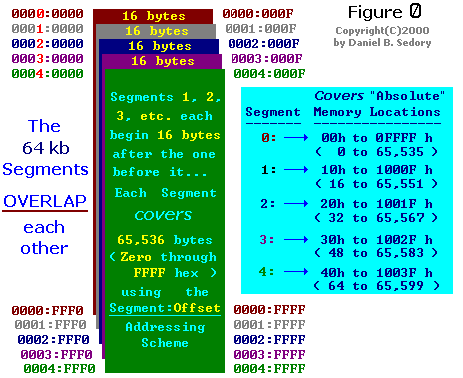
\includegraphics[width=0.5\textwidth]{../img/mem_seg}
  \label{fig:mem_seg} 
\end{figure}

هذا \textbf{التداخل \en{Overlapping}} سمح لأي برنامج ما إمكانية الوصول الى بيانات برنامج آخر والكتابة عليها وهذا ما جعل النمط الحقيقي ضعيف من ناحية حماية أجزاء الذاكرة.

\subsection{النمط المحمي \en{Protected Mode}}
بعد أن تم التعرف على هذه المشاكل سارعت أنتل باصدار المعالج \en{80286} والذي كان أول معالج يعمل في نمطين (الحقيقي والمحمي) . هذا المعالج (والمعالجات التي تليها) حل أهم مشكلة وهي حماية مقاطع الذاكرة من الوصول العشوائي من قبل برامج المستخدم وذلك عن طريق وصف مقاطع الذاكرة وصلاحيات الوصول اليها في جداول تسمى جداول الوصفات (\en{Descriptor Table}). المعالج \en{80386} هو أول معالج 32 بت ويستخدم مسجلات بحجم 32 يت وحجم مسار البيانات أيضا بنفس الحجم مما سمح بإمكانية التعامل مع ذاكرة بحجم 4 جيجابايت .كذلك تم اضافة دعم للذاكرة التخيلية ومفهوم الصفحات (\en{Paging}) ودعم تعدد المهام. وفي هذا البحث سيتم الحديث عن معالجات 32 بت باعتبارها أحد الأكثر انتشاراً حتى وقتنا هذا ،و على الرغم من ظهور معالجات 64 بت إلا ان الدراسة حول معالجات 32 بت تعتبر هي الأساس نظراً لان المعالجات الحديثة ما هي الا تطوير واضافات للمفاهيم الموجودة على المعالجات السابقة.

\subsubsection{حلقات المعالج \en{CPU Rings}}
عندما يعمل المعالج في النمط المحمي فان هذا يضمن حماية للذاكرة من برمجيات المستخدم ، وهذا بسبب توصيف الذاكرة وصلاحيات الوصول لها في جدول يستخدمه المعالج لعنونة الذاكرة وهو جدول الواصفات. نظام الصلاحيات الذي تم ادخاله الى المعالج عند عمله في النمط المحمي يسمى \textbf{بحلقات المعالج (\en{CPU Rings})}، هذه الحلقات تحدد مستوى الحماية المطلوب لكي يستخدمها المعالج في تقرير ما اذا كان تنفيذ أمر ما يحتاج الى صلاحية أعلى أم لا، وكذلك لكي يقرر ما اذا كان الوصول الى عنوان معين في الذاكرة مسموحٌ باستخدام صلاحية معينة أم لا.وتوجد أربع حلقات للمعالج تبدأ من الحلقة صفر (\en{Ring0}) وتنتهي بالحلقة 3 (\en{Ring3}). الحلقة صفر تسمى نمط النواة (\en{Kernel Mode}) بسبب أن أي برنامج يعمل في الحلقة صفر لديه الصلاحيات الكاملة على النظام بالوصول الى أي عنوان في الذاكرة وتنفيذ أي تعليمية حتى لو تسببت في ايقاف النظام عن العمل (المسؤولية تقع على البرنامج) لذلك غالبا البرامج التي تعمل في الحلقة صفر هي البرامج التي تتبع لنظام التشغيل. أما الحلقة 3 تسمى بنمط المستخدم (\en{User Mode}) حيث أن البرامج التي تعمل عليها لا تملك صلاحيات لتنفيذ العديد من الأوامر (مثل الامر \cmd{cli} والأمر \cmd{hlt}) ولا تملك الوصول الى أي عنوان في الذاكرة بخلاف مساحة العنونة التخيلية (\en{Virtual Address Space}) الخاصة بالبرنامج نفسه وهذا ما رفع درجة حماية الذاكرة الى أقصى حد ممكن ، والشكل \ref{fig:rings} يوضح هذه الحلقات وصلاحياتها. وعندما يبدأ النظام بالإقلاع فان المعالج يكون في النمط الحقيقي وهو نمط لا يحوي على حلقات حيث أنه يمكن تنفيذ كل الأوامر والوصول الى أي عنوان في الذاكرة ، وعند التحويل الى النمط المحمي (\en{PMode}) فان المعالج يكون في الحلقة صفر (\en{Kernel Mode}) ، ويتم تحويل الحلقة الى حلقة معينة تلقائيا عند نقل التنفيذ الى عنوان في الذاكرة موصوف في جدول الواصفات بأنه يعمل بتلك الحلقة.

\begin{figure}[h!]
  \caption{حلقات المعالج}
  \centering
   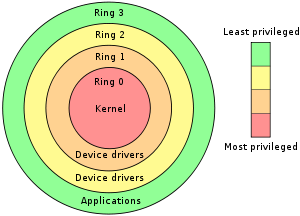
\includegraphics[width=0.5\textwidth]{../img/rings}
  \label{fig:rings} 
\end{figure}

\subsection{النمط الغير حقيقي والنمط التخيلي}


\subsection{معمارية معالجات \en{x86}}
أي معالج يتعرف على مجموعة من الأوامر تسمى \en{Instruction Set} بعضاً منها تتطلب صلاحية معينة (الحلقة صفر) لكي يقوم المعالج بتنفيذها (انظر الجدول \ref{tbl:ring0} لمعرفة هذه الأوامر) وإلا فان هذا سيتسبب في حدوث خطأ من المعالج يسمى الخطأ العام (\en{General Protection Fault}) والذي ان لم تتوفر دالة تتعامل معه (\en{Exception Handler}) فان هذا يؤدي الى توقف النظام عن العمل.

\begin{table}
\caption{الأوامر التي تتطلب صلاحية الحلقة صفر}
{تنفيذ هذه الأوامر من قبل برمجيات المستخدم يؤدي الى حدوث خطأ وتوقف النظام عن العمل في حالة لم تتوفر دالة تتعامل مع هذا الخطأ.}
\centering
\begin{tabular}{ | l | r |}
\hline  
الأمر & الوصف \\
\hline \hline
\en{LGDT} &  تحميل جدول الواصفات العام الى المسجل \en{GDTR} \\
\en{LLDT} & تحميل جدول الواصفات الخاص الى المسجل \en{LDTR} \\
\en{LTR} &  تحميل مسجل المهام \\
\en{MOV cr\_x} &  نقل بيانات الى مسجل تحكم \\
\en{LMSW} &  تحميل \en{new Machine Status WORD} \\
\en{MOV dr\_x} &  نقل بيانات الى مسجل تنقيح \\
\en{CLTS} & تصفير \en{Task Switch Flag} في مسجل التحكم الأول \\
\en{INVD} & \en{Invalidate Cache without writeback} \\
\en{INVLPG} & \en{Invalidate TLB Entry} \\
\en{WBINVD} &\en{Invalidate Cache with writeback} \\
\en{HLT} &  إيقاف عمل المعالج \\
\en{RDMSR} & قراءة مسجل \en{MSR} \\
\en{WRMSR} & الكتابة الى مسجل \en{MSR} \\
\en{RDPMC} & قراءة \en{Performance Monitoring Counter} \\
\en{RDTSC} &  قراءة \en{time Stamp Counter} \\
 \hline  
\end{tabular}
\label{tbl:ring0}
\end{table}

وتحوي معالجات \en{x86} العديد من المسجلات منها ما يستخدم للأغراض العامة (\en{General Registers})  ومنها ما يستخدم لحفظ العناوين وأرقام المقاطع (\en{Segments Registers}) وتوجد أيضا مسجلات لا يمكن استخدامها إلا في برامج الحلقة صفر (أي النواة) حيث أن التغيير فيها يؤثر على عمل النظام وأخيرا هناك مجموعة من المسجلات الداخلية للمعالج والتي لا يمكن الوصول لها برمجياً. والقائمة التالية توضح هذه المسجلات :

\begin{itemize}
\item مسجلات عامة : \en{RAX (EAX(AX/AH/AL)), RBX (EBX(BX/BH/BL)), RCX (ECX(CX/CH/CL)), RDX (EDX(DX/DH/DL))}.
\item مسجلات عناوين:
\begin{itemize}
\item مسجلات مقاطع:\en{ CS,SS,ES,DS,FS,GS}.
\item مسجلات إزاحة: \en{RSI (ESI (SI)), RDI (EDI (DI)), RBP (EBP (BP)). RSP (ESP (SP)), RIP (EIP (IP))}.
\end{itemize}
\item مسجل الأعلام: \en{RFLAGS (EFLAGS (FLAGS))}.
\item مسجلات التنقيح: \en{DR0, DR1, DR2, DR3, DR4, DR5, DR6, DR7}.
\item مسجلات التحكم: \en{CR0, CR1, CR2, CR3, CR4, CR8}.
\item مسجلات الإختبار: \en{TR1, TR2, TR3, TR4, TR5, TR6, TR7}.
\item مسجلات أخرى: \en{mm0, mm1, mm2, mm3, mm4, mm5, mm6, mm7, xmm0, xmm1, xmm2, xmm3, xmm4, xmm5, xmm6, xmm7, GDTR, LDTR, IDTR, MSR, and TR}.
\end{itemize}

\subsubsection{المسجلات العامة \en{General Purpose Registers}}
في المعالجات 32 بت يوجد 4 أربع مسجلات عامة طول كل منها هو 32 بت (4 بايت) وتقسم أي من هذه المسجلات الى جزئين: الجزء الأعلى (\en{High Order Word}) وهو بطول 16 بت والجزء الأدنى (\en{Low Order Word}) وهو أيضا بطول 16 بت ، كذلك يُقسم الجزء الأدنى الى جزئين: الجزء الأعلى (\en{High Order Byte}) وهو بطول 8 بت والجزء الأدنى (\en{Low Order Byte}) وهو أيضا بطول 8 بت. على سبيل المثال مسجل \en{EAX} حيث يقسم الى جزء أعلى (لا يمكن الوصول اليه بشكل مباشر) وجزء أسفل وهو  \en{AX} الذي يُقسم أيضا الى قسمين \en{AH} و \en{AL}. كل مسجل من هذه المسجلات العامة يستخدم لأي شيء لكن هناك بعض الإستخدامات الغالبة لكلٌ منهم توضحها القائمة التالية.

\begin{itemize}
\item المسجل \en{EAX}: يستخدم لنقل البيانات والعمليات الحسابية.
\item المسجل \en{EBX}: يستخدم في الوصول للذاكرة بشكل غير مباشر وذلك باستخدام مسجل آخر يعمل كعنوان رئيسي \en{Base Address}.
\item المسجل \en{ECX}: يستخدم في عمليات التكرار والعد.
\item المسجل \en{EDX}: يستخدم في تخزين البيانات.
\end{itemize}

\subsubsection{مسجلات المقاطع \en{Segment Registers}}
مسجلات المقاطع تستخدم لتخزين أرقام وعناوين المقاطع (\en{Segments}) وتوجد 6 مسجلات مقاطع تستخدم في النمط الحقيقي كما يلي:

\begin{itemize}
\item المسجل \en{CS}: يحوي عنوان بداية مقطع الشفرة للبرنامج المراد تنفيذه.
\item المسجل \en{DS}: يحوي عنوان بداية مقطع البيانات للبرنامج المراد تنفيذه.
\item المسجل \en{SS}: يحوي عنوان بداية مقطع المكدس للبرنامج المراد تنفيذه.
\item المسجل \en{ES}: يحوي عنوان بداية مقطع البيانات للبرنامج المراد تنفيذه.
\item المسجل \en{FS}: يحوي عنوان مقطع بعيد.
\item المسجل \en{GS}: يستخدم للأغراض العامة.
\end{itemize}

أما في النمط المحمي (\en{PMode}) فإن هذه المسجلات لا تشير الى مقاطع البرامج والبيانات وإنما تشير الى واصفات معينة في جدول الواصفات العام ، هذه الواصفات تحدد عنوان بداية المقطع ونوع المقطع (يحوي شفرات أم بيانات ) وتحدد صلاحية التنفيذ وصلاحية والقراءة والكتابة فيها - كما سنرى ذلك في الفصل الرابع بإذن الله-.

\subsubsection{مسجلات الإزاحة \en{Offset Registers}}
 بجانب مسجلات المقاطع فإن الوصول الى الذاكرة في النمط الحقيقي يتطلب عنوان الإزاحة بداخل المقطع ، وتوجد 4 مسجلات إزاحة في معالجات \en{x86} حجم كل منها هو 32 بت في الأنظمة 32 بت و 16 بت في أنظمة 16 بت. والقائمة التالية توضح هذه المسجلات:

\begin{itemize}
\item المسجل \en{SI}: يحوي عنوان الإزاحة في مقطع البيانات.
\item المسجل \en{DI}: نفس الوظيفة السابقة.
\item المسجل \en{BP}: يحوي عنوان الإزاحة بداخل مقطع المكدس ويمكن استخدام للأشارة على أي عنوان في أي مقطع آخر.
\item المسجل \en{SP}: يحوي عنوان الإزاحة بداخل مقطع المكدس.

\end{itemize}


\subsubsection{مؤشر التعليمة \en{Instruction Pointer}}
هذا المسجل (\en{IP}) يمثل إزاحة بداخل مقطع الشفرة (\en{CS}) وهو يحوي عنوان التعليمة التالية التي سيقوم المعالج بتنفيذها ، والعنوان \en{CS:IP} يمثل العنوان الفيزيائي للتعليمة التالية. هذا المسجل هو بطول 32 بت (\en{EIP}) في أنظمة 32 بت و 16 بت (\en{IP}) في أنظمة 16 بت، وهو مسجل لا يمكن تغيير محتواه باستخدام تعليمة المعالج \en{MOV} وإنما يتم تغيير محتواه عن القفز الى مكان آخر للتنفيذ.

\subsubsection{مسجل الأعلام \en{FLAGS Register}}
مسجل الأعلام هو مسجل بحجم 32 بت (\en{EFLAGS}) في أنظمة 32 بت و بحجم 16 بت (\en{FLAGS}) في أنظمة 16 بت ، وهذا المسجل هو عبارة عن بتات (بالحجم السابق ذكره) كل بت لديه وظيفه محدده ، وينقسم بشكل عام الى \textbf{بتات حالة (\en{Status})} بحيث تعكس حالة الأوامر التي يقوم المعالج بتنفيذها و \textbf{بتات تحكم (\en{Control})} بحيث تتحكم في بعض الخصائص و \textbf{بتات للنظام (\en{System})}. والجدول \ref{tbl:eflags} يوضح وظيفة كل بت في هذا المسجل.


\begin{table}
\caption{مسجل الأعلام \en{EFLAGS}}
\centering
\begin{tabular}{ | r | r | r |}
\hline  
رقم البت & اسم البت & الإستخدام \\
\hline \hline
\en{0} & \en{CF} & \en{Carry Flag - Status bit} \\
\en{1} & \en{-} & محجوزة \\
\en{2} & \en{PF} & \en{Parity Flag} \\
\en{3} & \en{-} & محجوزة \\
\en{4} & \en{AF} & \en{Adjust Flag - Status bit} \\
\en{5} & \en{-} & محجوزة \\
\en{6} & \en{ZF} & \en{Zero Flag - Status bit} \\
\en{7} & \en{SF} &  \en{Sign Flag - Status bit} \\
\en{9} & \en{TF} &  \en{Trap Flag - System Flag} \\
\en{9} & \en{IF} &  \en{Interrupt Enabled Flag - System Flag} \\
\en{10} & \en{DF} & \en{Direction Flag - Control Flag} \\
\en{11} & \en{OF} &  \en{Overflow Flag - Status bit} \\
\en{12-13} & \en{IOPL} & \en{I/O Priviledge Level  - Control Flag} \\
\en{14} & \en{NT} & \en{Nested Task Flag - Control Flag} \\
\en{15} & \en{-} & محجوزة \\
\en{16} & \en{RF} & \en{Resume Flag (386+ Only) - Control Flag} \\
\en{17} & \en{VM} & \en{v8086 Mode Flag (386+ Only) - Control Flag} \\
\en{18} &\en{ AC} & \en{Alignment Check (486SX+ Only) - Control Flag} \\
\en{19} & \en{VIF} & \en{Virtual Interrupt Flag (Pentium+ Only) - Control Flag} \\
\en{20} & \en{VIP} & \en{Virtual Interrupt Pending (Pentium+ Only) - Control Flag} \\
\en{21} & \en{ID} & \en{Identification (Pentium+ Only) - Control Flag} \\
\en{22-31} & \en{-} & محجوزة \\
 \hline  
\end{tabular}
\label{tbl:eflags}
\end{table}

ويحدد البتين \en{IOPL} مستوى الحماية المطلوب لتنفيذ مجموعة من الأوامر (مثل الأوامر \en{CLI,STI,IN,OUT}) حيث لن يتم تنفيذ مثل هذه التعليمات إلا في حالة كان مستوى الحماية الحالي \en{Current Priviledge  Level} أعلى من أو مساوياً للقيمة الموجودة في البتين \en{IOPL}\footnote{أعلى مستوى حماية هو الحلقة صفر (\en{Ring0}) ويليها الحلقة 1 ثم 2 و3.} ، وغالباً ما تكون القيمة هي صفر دلالة على أن التعليمات السابقة لا يتم تنفيذها الا لبرامج النواة (\en{Ring0}).  


\subsubsection{مسجلات التحكم \en{Control Registers}}
توجد في معالجات 32 بت ستة مسجلات للتحكم في سلوك وعمل المعالج وهي \en{CR0, CR1, CR2,CR3, CR4, CR8} ، ونظراً لخطورة التعامل معها فان هذه المسجلات لا يمكن الوصول لها إلا عند العمل في نمط النواة (\en{Kernel Moder/Ring0}) ولا يُمكن لبرمجيات المستخدم الوصول الى هذه المسجلات والتعامل معها. وفي الوقت الحالي يهمنا فقط أول مسجل تحكم وهو \en{CR0} حيث من خلاله يمكن أو نقوم بعملية تحويل نمط المعالج من النمط الحقيقي الى النمط المحمي (\en{PMode}) وكذلك يمكن أن نقوم بتفعيل خاصية الصفحات (\en{Paging}) ، والتركيبة التالية توضح محتويات كل بت في مسجل التحكم \en{CR0} وهو مسجل بحجم 32 بت.

\begin{english}
\fontspec[Scale=1.2,Mapping=englishdigits]{Calibri}

\begin{itemize}
\item Bit 0 (PE) : \textbf{Puts the system into protected mode.}
\item  Bit 1 (MP) : Monitor Coprocessor Flag This controls the operation of the WAIT instruction.
\item Bit 2 (EM) : Emulate Flag. When set, coprocessor instructions will generate an exception
\item Bit 3 (TS) : Task Switched Flag This will be set when the processor switches to another task.
\item Bit 4 (ET) : ExtensionType Flag. This tells us what type of coprocesor is installed.
\begin{itemize}
\item 0 - 80287 is installed
\item 1 - 80387 is installed.
\end{itemize}
\item Bit 5 (NE): Numeric Error
\begin{itemize}
\item 0 - Enable standard error reporting
\item 1 - Enable internal x87 FPU error reporting
\end{itemize}
\item  Bits 6-15 : Unused
\item Bit 16 (WP): Write Protect
\item Bit 17: Unused
\item Bit 18 (AM): Alignment Mask
\begin{itemize}
\item 0 - Alignment Check Disable
\item 1 - Alignment Check Enabled (Also requires AC flag set in EFLAGS and ring 3)
\end{itemize}
\item Bits 19-28: Unused
\item Bit 29 (NW): Not Write-Through
\item Bit 30 (CD): Cache Disable
\item Bit 31 (PG) : \textbf{Enables Memory Paging.}
\begin{itemize}
\item 0 - Disable
\item 1 - Enabled and use CR3 register
\end{itemize}

\end{itemize}
\end{english}


\end{document}
